\documentclass[11pt, aspectratio=169]{beamer}

\usepackage[utf8]{inputenc}
\usepackage{tikz}
\usepackage[english]{babel}
\usepackage{svg}
\usepackage{eurosym}
\usepackage{subfig}
\usepackage{pgfgantt}
\usepackage[export]{adjustbox}
%\usepackage[shortlabels]{enumitem}
\usepackage[font=scriptsize,justification=centering]{caption}
\usepackage{movie15}
\usepackage{tikz}
\usetikzlibrary{arrows,shapes,positioning,shadows,trees}
\graphicspath{{figures/}}

%----------------------------------------------------------------------------------------
%	TITLE PAGE INFORMATION.
%----------------------------------------------------------------------------------------
\author{S. Björk, J. Hooper, J. M. Inga, H. Magnusson, A. Śmiałek}
\title{InfraRed Imaging of astronomical targets with a Stabilised Camera}
\subtitle{IRISC}
\institute{ESA ESTEC, Noordwijk}
\date{13-17 April 2019}
%\subject{} 

%----------------------------------------------------------------------------------------
%	SETUP LAYOUT.
%----------------------------------------------------------------------------------------
\usepackage{theme/beamerthemeWarsawLTU}
%\usetheme{Warsaw}


\begin{document}
%----------------------------------------------------------------------------------------
%	TITLE PAGE.
%----------------------------------------------------------------------------------------

{\setbeamertemplate{logo}{}
\begin{frame}
\titlepage
\begin{tikzpicture}[remember picture,overlay]
    \node[xshift=13cm,yshift=-1.025\textheight,anchor=north west] at (current page.north west){%
    
\includegraphics[width=2cm]{theme/LTU_logo.jpg}};
\end{tikzpicture}
\end{frame}
}

%----------------------------------------------------------------------------------------
%	TABLE OF CONTENTS.
%----------------------------------------------------------------------------------------
\begin{frame}[t]{Table of Contents}
\vspace{-0.3cm}
    \begin{columns}[t]
        \begin{column}{.5\textwidth}
            \tableofcontents[sections={1-2}]
        \end{column}
        \begin{column}{.5\textwidth}
            \tableofcontents[sections={3-5}]
            \vspace{-.2cm}
            \tableofcontents[sections=6,hidesubsections]
        \end{column}
    \end{columns}
\end{frame}


%----------------------------------------------------------------------------------------
%	INTRODUCTION.
%----------------------------------------------------------------------------------------

%----------------------------------------------------------------------------------------
%	SCIENCE.
%----------------------------------------------------------------------------------------
\section{Science}

%----------------------------------------------------------------------------------------
%	SYSTEM.
%----------------------------------------------------------------------------------------
\section{System}
%	CONSTRUCTION. -----------------------------------------------------------------------
\subsection{Construction}
%	THERMAL. ----------------------------------------------------------------------------
\subsection{Thermal}
%	ELECTRICAL. -------------------------------------------------------------------------
\subsection{Electrical Setup}
%	SOFTWARE. ---------------------------------------------------------------------------
\subsection{On-board Software}
%	GROUND STATION?. --------------------------------------------------------------------
\subsection{Ground Station}
%	CONTROL. ----------------------------------------------------------------------------
\subsection{Control System}

\begin{frame}{Control system}
    Objectives of the control system:
    \begin{itemize}
        \item Selection and tracking the astronomical targets
        \item Stabilisation the telescope during exposure
        \item Avoid pointing the telescope at the Sun
        \item Thermal control of the CMOS sensor and the electronics box
    \end{itemize}
\end{frame}

\begin{frame}{Control system}
    \begin{itemize}
        \item<1-> Selection of targets: %\\
        \begin{itemize}
            \item Based on prioritisation parameters (e.\,g. brightness, location)
            \item Sensor data: star tracker, GPS %\\
        \end{itemize}
        \item<2-> Tracking of targets: 
        \begin{itemize}
            \item Model of movements of astronomical targets
            \item Sensor data: internal clock, GPS
        \end{itemize}
        \item<3-> Stabilisation of the gimbal: dynamic control system (PID) %\\
        \begin{itemize}
            \item Mechanical model of the gimbal, motors model
            \item Sensor data: gyroscopes, encoders%\\
        \end{itemize}
        \item<4-> Feedback loop, measured states: 
        \begin{itemize}
            \item Kalman filter determines exact position \& orientation
        \end{itemize}
    \end{itemize}
\end{frame}

\begin{frame}[t]{Control system}
    \begin{figure}
        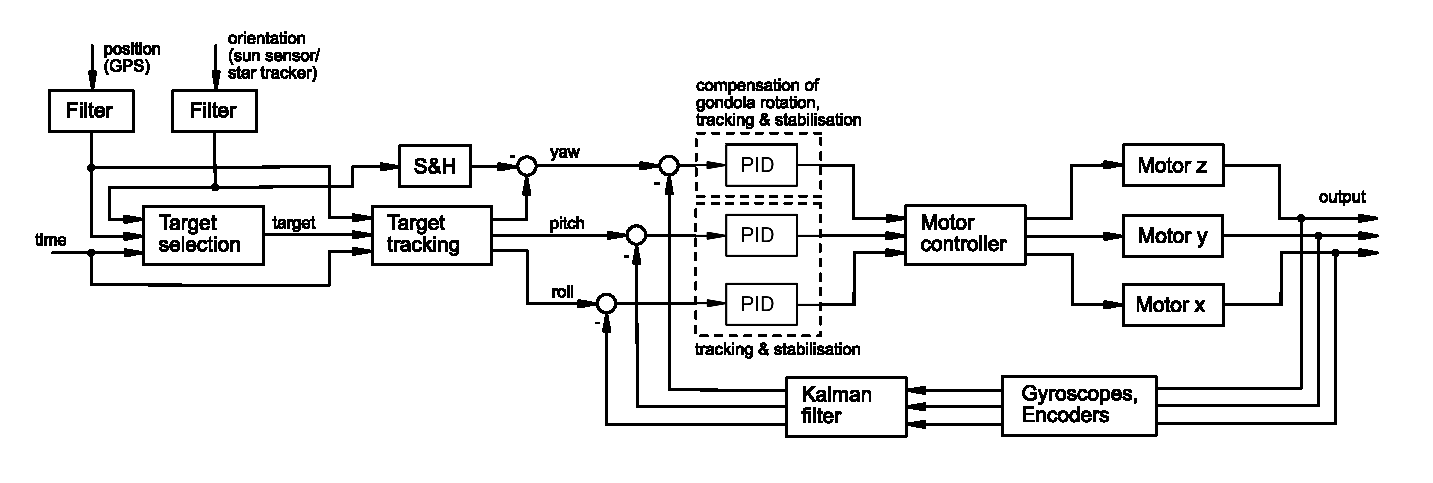
\includegraphics[width=\linewidth]{figures/images/Control_loop.eps}
        \caption{Main control loop}
    \end{figure}
\end{frame}

%	CAMERA. -----------------------------------------------------------------------------
\subsection{Cameras}
%	TELESCOPE. --------------------------------------------------------------------------
\subsection{Telescope}

%----------------------------------------------------------------------------------------
%	REQUIREMENTS AND RISKS.
%----------------------------------------------------------------------------------------
\section{Requirements and risks}
%	REQUIREMENTS. -----------------------------------------------------------------------
\subsection{Requirements}
%	RISKS. ------------------------------------------------------------------------------
\subsection{Risks}

%----------------------------------------------------------------------------------------
%	PROJECT MANAGEMENT.
%----------------------------------------------------------------------------------------
\section{Project Management}
%	TEAM. ---------------------------------------------------------------------------
\subsection{Team composition}

\begin{frame}{Team composition}
    \begin{figure}
        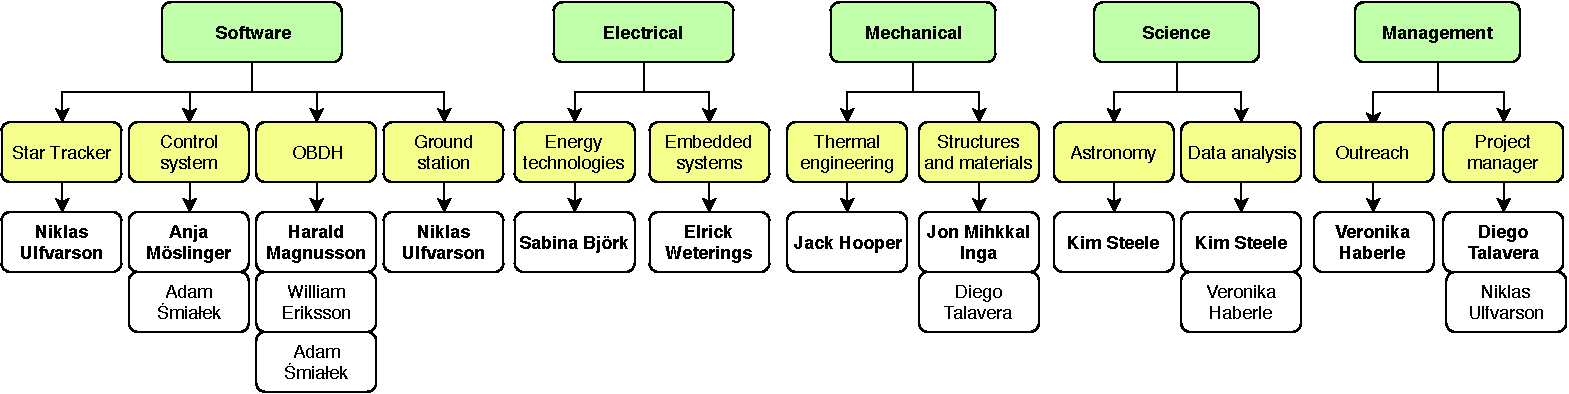
\includegraphics[width=\linewidth]{images/Team_structure.pdf}
        \caption{Work breakdown structure}
    \end{figure}
\end{frame}

\begin{frame}{Project schedule}
    \begin{figure}
        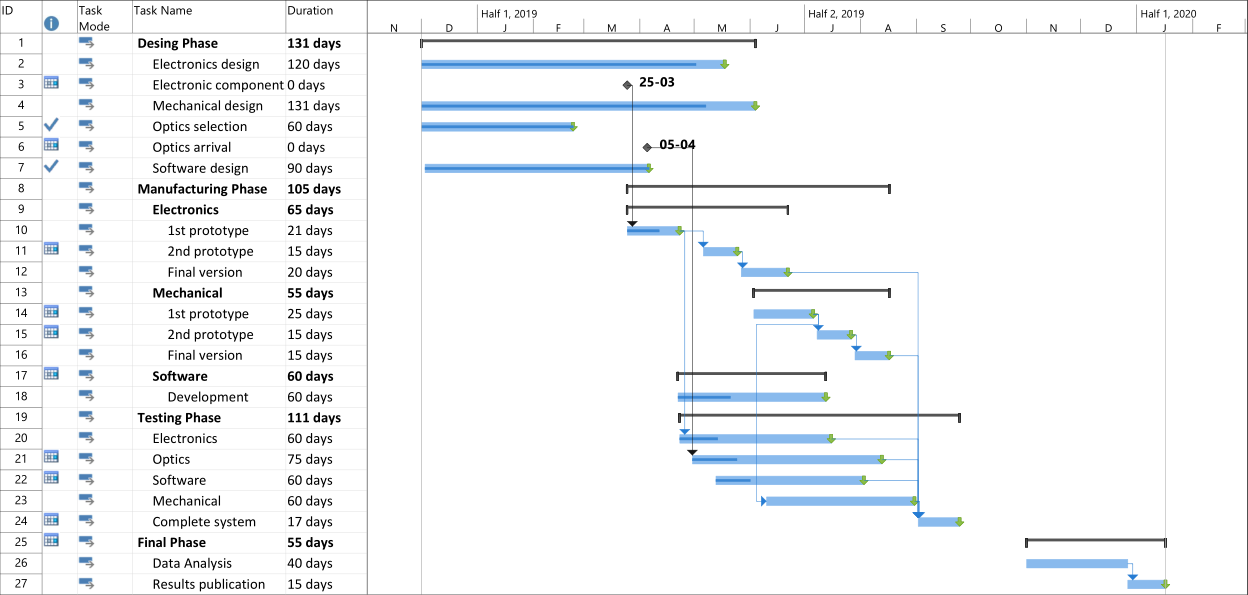
\includegraphics[width=0.98\linewidth]{images/gantt.png}
        \caption{Work breakdown structure}
    \end{figure}
\end{frame}

%	PLANNING. ---------------------------------------------------------------------------
\subsection{Time planning}
%	BUDGET. -----------------------------------------------------------------------------
\subsection{Budget}
%	OUTREACH. ---------------------------------------------------------------------------
\subsection{Outreach}

%----------------------------------------------------------------------------------------
%	SUMMARY.
%----------------------------------------------------------------------------------------
\section{Summary}

%----------------------------------------------------------------------------------------
%	QUESTIONS.
%----------------------------------------------------------------------------------------
\section{Questions}

%\begin{frame}[plain]{}
%%    \label{slide:questions}
%%    \centering
%%    \vspace{-0.71cm}
%%    \begin{figure}
%%    \hspace*{-1.1cm}
%%    	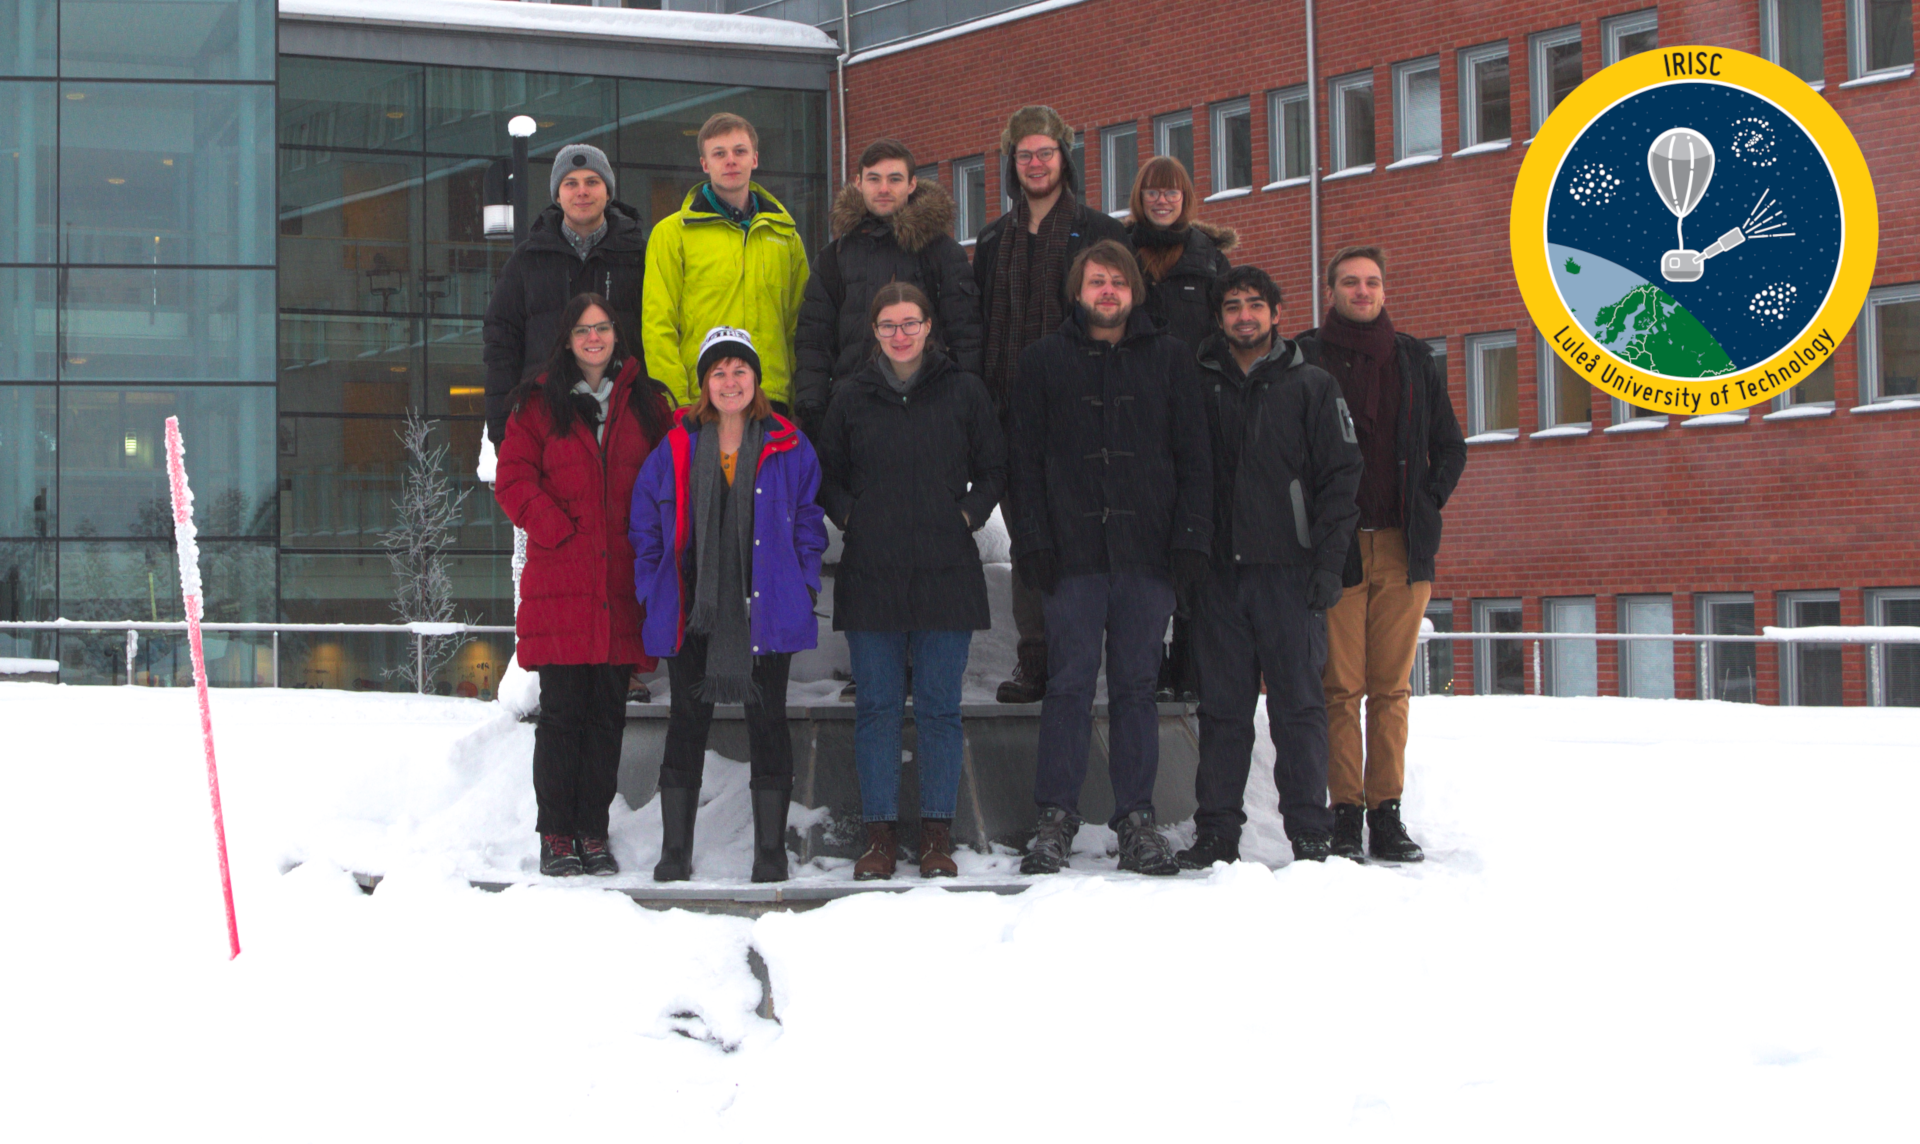
\includegraphics[width=1.15\textwidth]{figures/images/teamphoto.png}
%%    \end{figure}
%	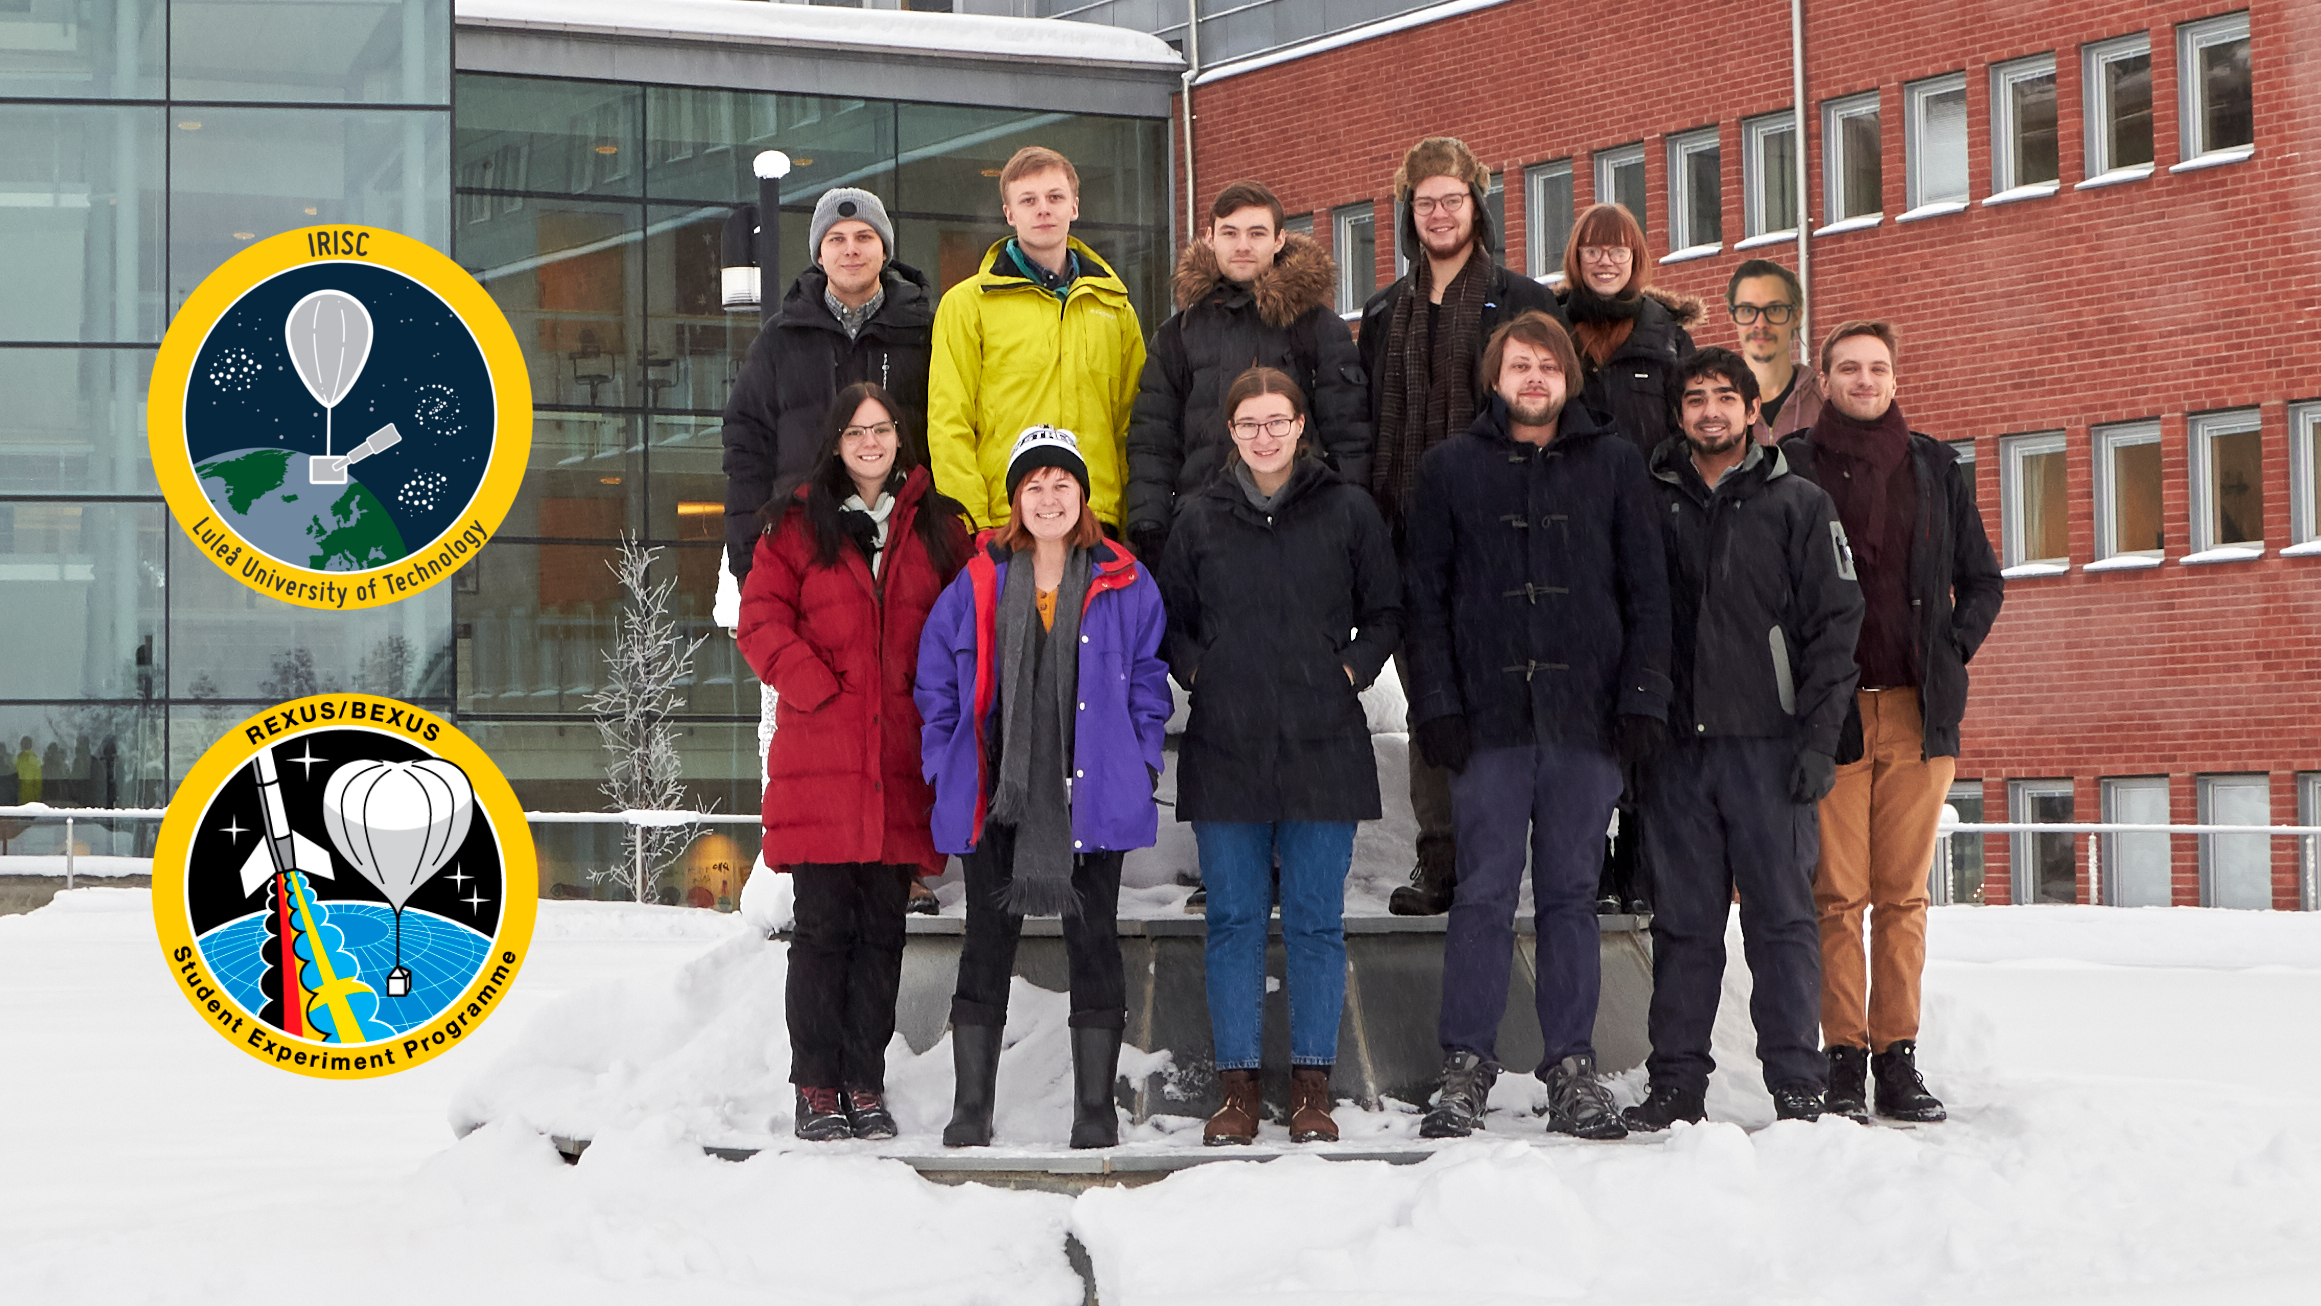
\includegraphics[width=\paperwidth]{figures/images/IRISC_Team_001_16_9+logo.jpg}
%\end{frame}
{
\usebackgroundtemplate{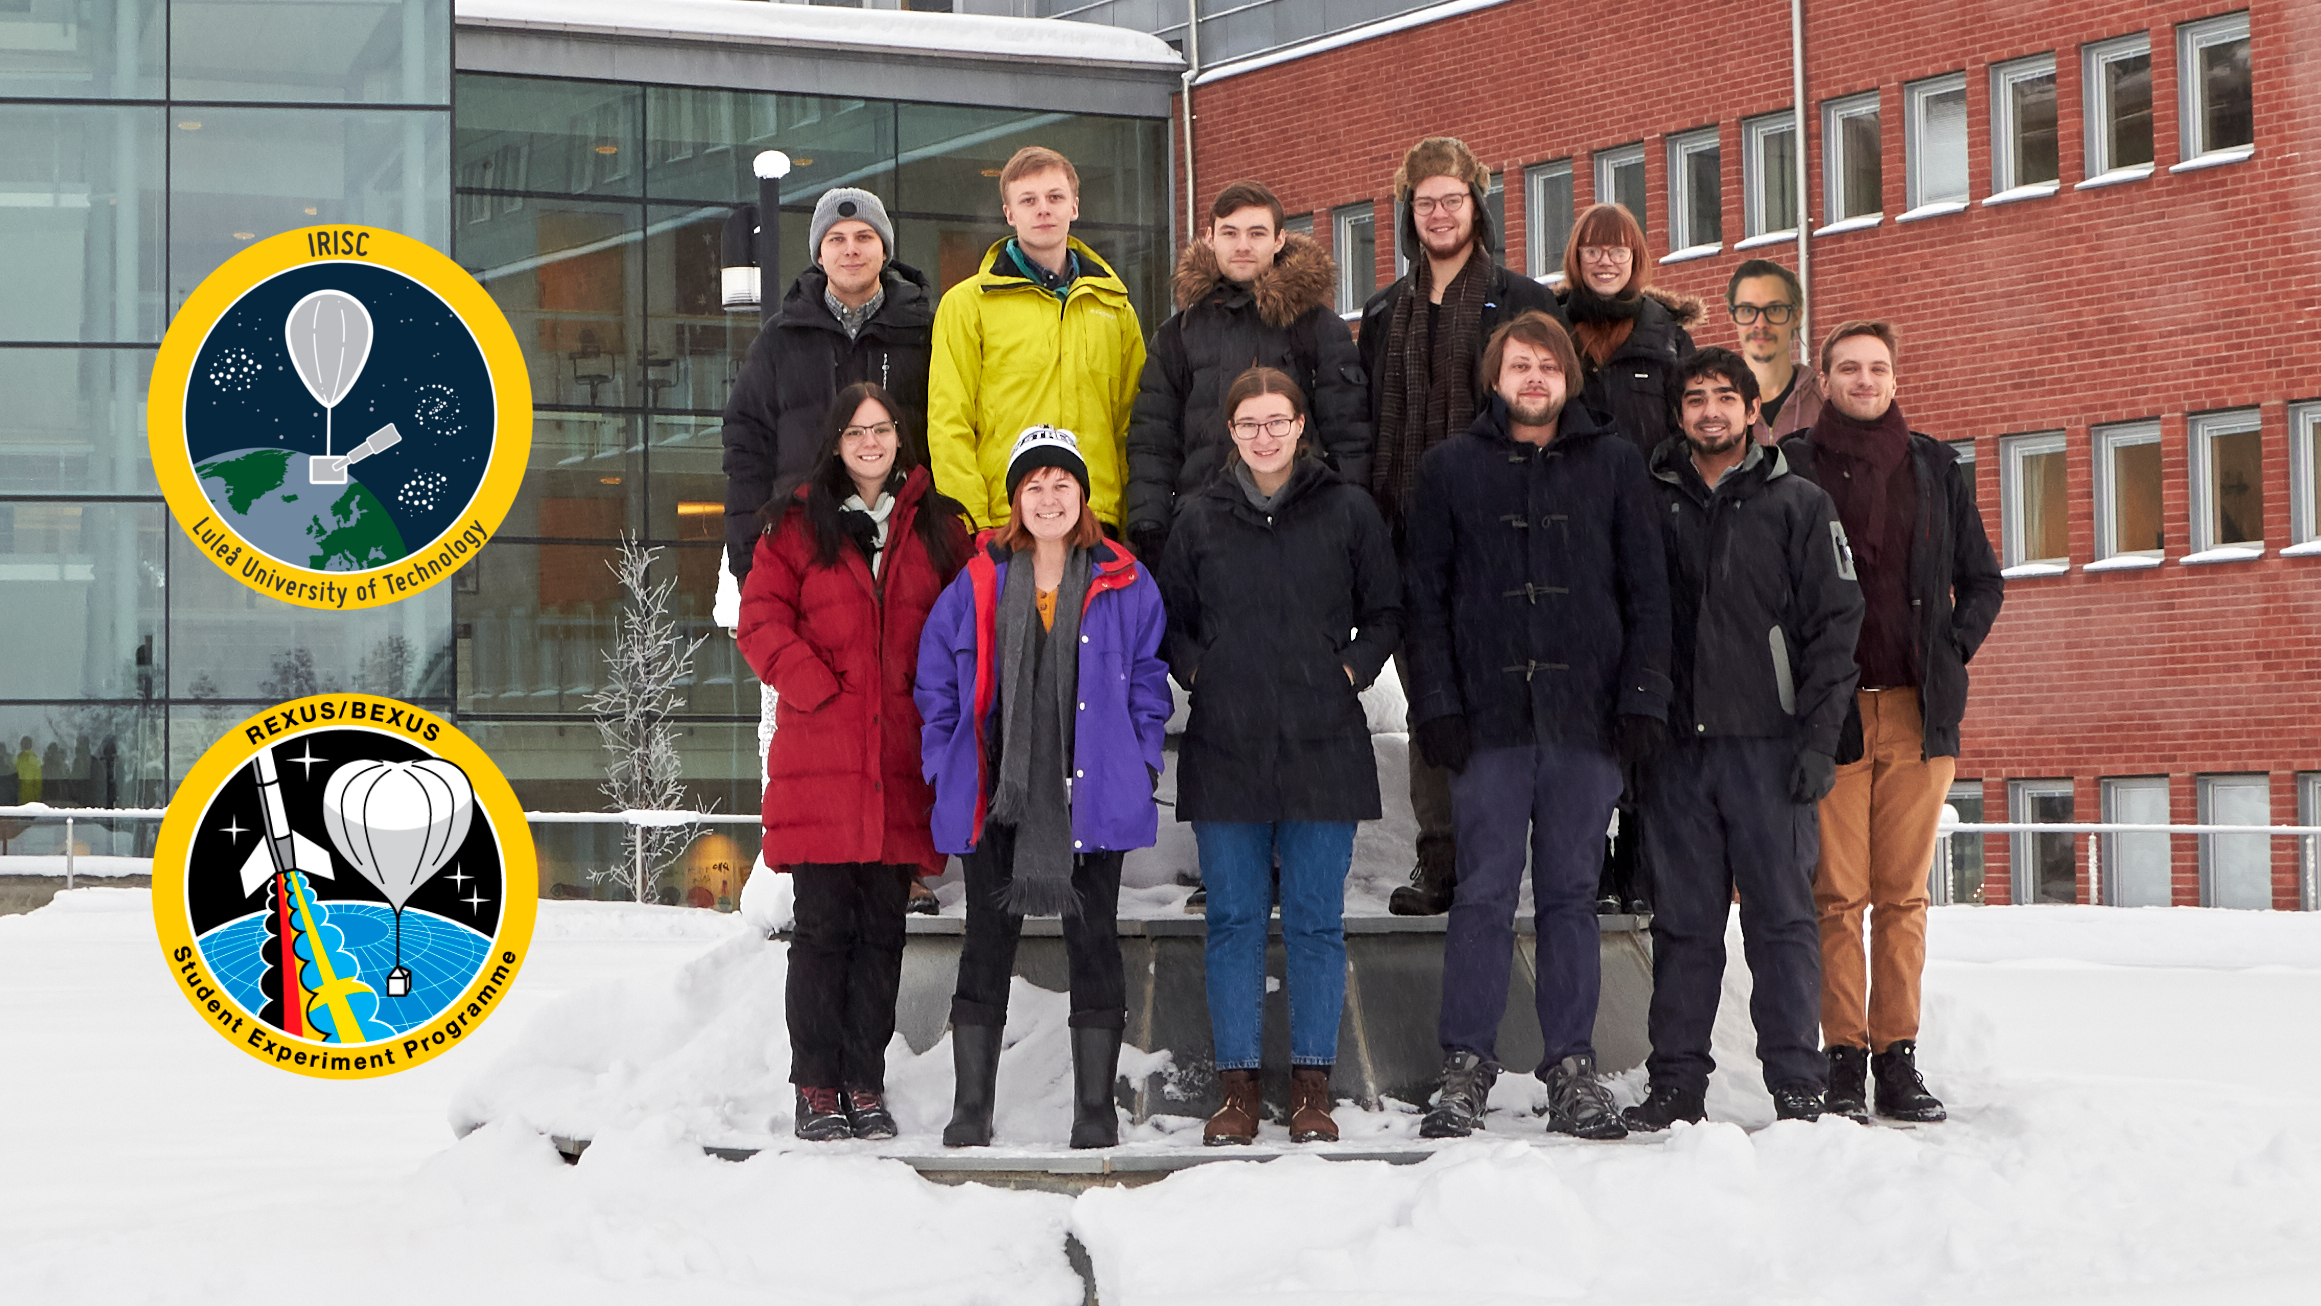
\includegraphics[width=\paperwidth]{figures/images/IRISC_Team_001_16_9+logo.jpg}}
\begin{frame}[plain]
%\label{slide:questions}
\end{frame}

}
%----------------------------------------------------------------------------------------
%	BACKUP SLIDES. 				EVERYONE!!!
%----------------------------------------------------------------------------------------

\end{document}
